\documentclass{article}
%\usepackage[latin1]{inputenc}
\usepackage{graphicx,amssymb,amsmath,amsbsy,MnSymbol} % extensions pour maths avancées
\usepackage{graphicx,mathenv}           % extensions pour figures
\usepackage[T1]{fontenc}        % pour les charactères accentués 
\usepackage[utf8]{inputenc} 
\usepackage{multicol}
\usepackage{wrapfig}
\usepackage{stmaryrd} % Pour les crochets d'ensemble d'entier
\usepackage{float}  % Pour placer les images là ou JE veux.

\DeclareMathOperator{\tr}{tr}
\DeclareMathOperator{\argmax}{argmax}


\setlength{\parindent}{0.0in}
\setlength{\parskip}{0.1in}
\setlength{\topmargin}{-0.4in}
\setlength{\topskip}{0.7in}    % between header and text
\setlength{\textheight}{9in} % height of main text
\setlength{\textwidth}{6in}    % width of text
\setlength{\oddsidemargin}{0in} % odd page left margin
\setlength{\evensidemargin}{0in} % even page left margin
%
%% Quelques raccourcis clavier :
\def\slantfrac#1#2{\kern.1em^{#1}\kern-.3em/\kern-.1em_{#2}}
\def\b#1{\mathbf{#1}}
\def\bs#1{\boldsymbol{#1}}
\def\m#1{\mathrm{#1}}
\bibliographystyle{plain}
%
\newcommand{\greeksym}[1]{{\usefont{U}{psy}{m}{n}#1}}
\newcommand{\inc}{\mbox{\small\greeksym{d}\hskip 0.05ex}}%
\pagenumbering{arabic}
\date{\today}
\title{L'utilisation du MeanShift pour la segmentation d'image}
\author{Nelle Varoquaux}
\begin{document}
\maketitle

\begin{abstract} \textit{Peu connu de la littérature, l'algorithme Mean Shift
présente un interêt particulier pour les tâches de vision impliquant une étude
d'un espace de caractères ou descripteurs. \cite{my_article} remet au goût du
jour cet algorithme en 2002. Nous présentons ici une étude détaillée celui-ci
Mean Shift, ainsi qu'une application à la segmentation de l'image, telle que
décrit dans \cite{my_article}} \end{abstract}

\section{Introduction}

\begin{figure}
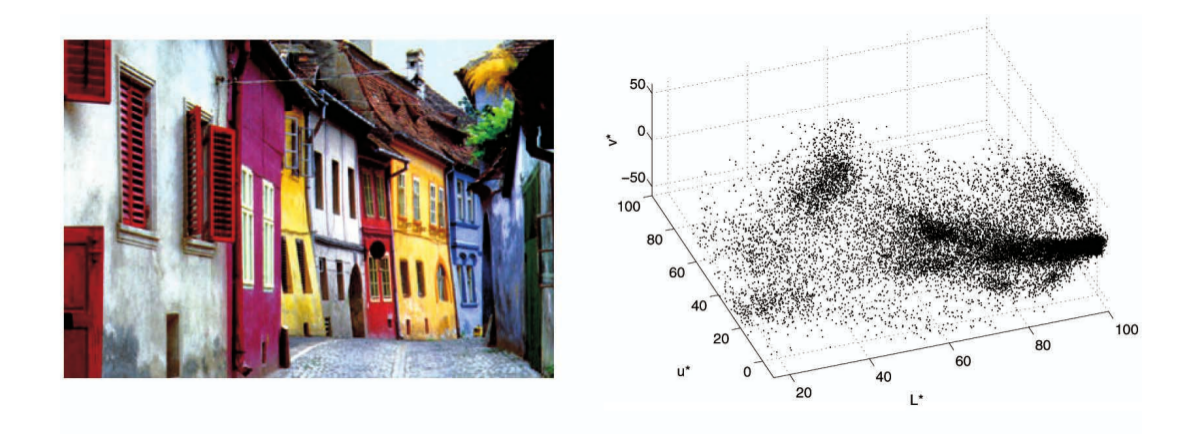
\includegraphics[width=400px]{images/color_space.png}
\end{figure}

De nombreuses tâches de vision bas niveau nécessite l'étude d'un espace des
caractéristiques, ou des descripteurs. De nombreuses techniques reposent sur
une bonne évaluation des paramètres: ceux-ci sont souvent devinés. \\
Un espace de paramètres est obtenu en étudiant localement une image: l'image
d'entrée peut par exemple être découpée en patchs, qui sont eux même
prétraiter. Des descripteurs sont extraits, et associé à un point dans
l'espace: le milieu du patch. Une fois que toute l'image est traité, on peut
obtenir les descripteurs les plus significatifs, les descripteurs
contenant le plus d'information,  en calculant les régions les plus denses de
l'espace de descripteurs: ces régions correspondent à des clusters. \\
La nature des descripteurs dépendent de l'application cherchée: cela peut être
des descripteurs locaux à un pixel, telle que une représentation des couleurs,
ou des descripteurs calculés à partir d'un petit patch de l'image,
représentant une texture. \\
L'analyse de cette espace varie elle aussi selon la tâche à effectuer. Malgré
le nombre important d'algorithmes de clustering, peu d'entre eux sont adaptés à
l'étude d'un espace de descripteurs: beaucoup reposent sur une connaissance
préalable du nombre de clusters ou de la forme de ceux-ci, ou alors sont mal
adpatés à l'étude d'un espace de descripteurs trop complexe, ce qui est
souvent le cas dans le domaine du traitement d'image. Parmi les algorithmes de
clustering les plus standards, on peut citer le k-means, qui nécessite une
connaissance du nombre de cluster, et les algorithmes hiérarchiques, qui
consiste à agréger des clusters entre eux, ou a les séparer, trop peu
efficace pour le traitement d'image. \\
On présente ici une détection de mode, maxima locaux d'une estimation non
paramétrique de densité de probabilité du noyau grâce à l'algorithme meanshift.


\section{Mean shift}

\begin{figure}
\begin{center}
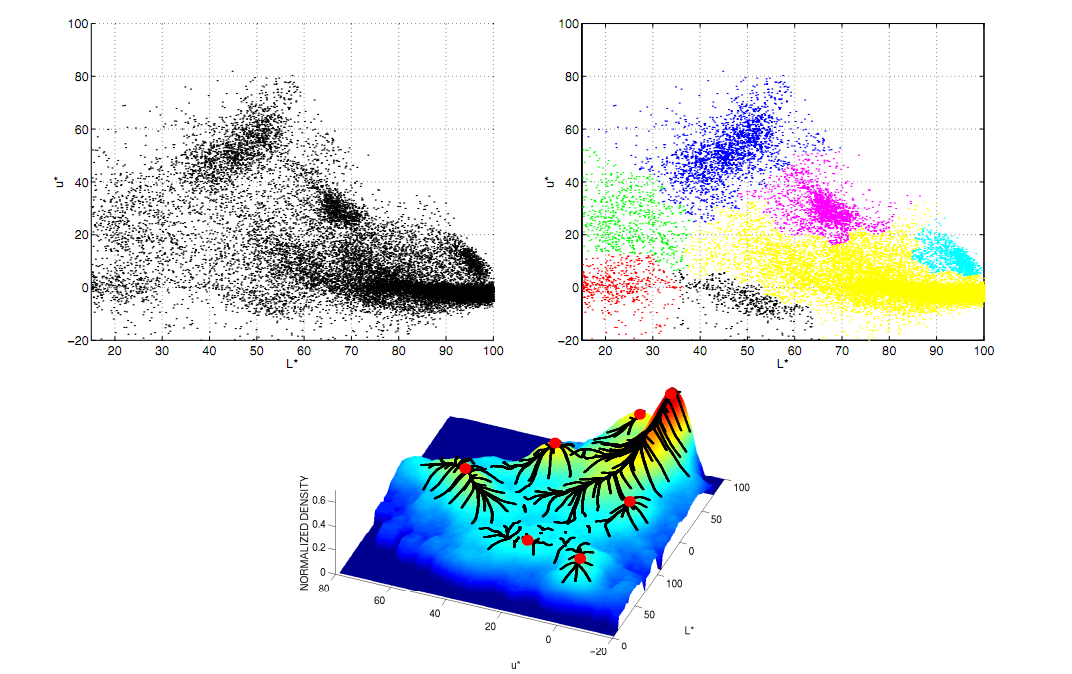
\includegraphics[width=400px]{images/mean_shift_color_space.png}
\end{center}
\end{figure}


L'algorithme de clustering Mean Shift ne nécessite pas la connaissance au
préalable du nombre de cluster, ni la forme des clusters. Présenté pour la
première fois par \cite{fukugana} en 1975, le mean shift est un estimateur non
paramétrique du gradient de la densité de probabilité. Disparu de la
littérature, il est remis au goût du jour par \cite{cheng} en 1995. Une
application au filtrage et à la segmentation est ensuite proposée en 1997,
1999 dans \cite{comaniciu_meer}. Il est ensuite utilisé dans des domaines tels
que le suivi d'objet, le maillage, et la segmentation d'image. Cette grande
variété d'application s'explique par l'exploitation de l'espace des
descripteurs. \\
L'algorithme repose sur la recherche de maximum d'une densité de probabilité,
\textit{un mode}. Une région est caractérisée par une densité de probabilité,
elle même représentée par un mode. Plusieurs régions impliquent donc plusieurs
modes. Trouver à quelle région appartient une donnée correspond donc à trouver
le mode de cette donnée.

\begin{itemize}
\item Déterminer aléatoirement des régions d'intérêt
\item Déterminer les centroïdes des régions
\item Recalculer les régions d'intérêt autour des centroïdes
\item Répéter les étapes jusqu'à la convergence
\end{itemize}

\begin{figure}
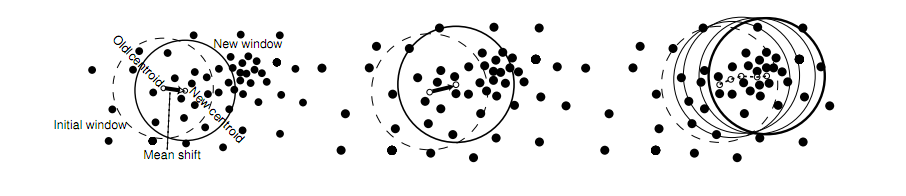
\includegraphics[width=400px]{images/mean_shift_proc.png}
\end{figure}

On note $K(\mathbf{x})$ le noyau, qui indique comment $\mathbf{x}$ contribue à
l'estimation de la moyenne. On peut alors calculer la moyenne $\mathbf{m}$ de
$\mathbf{x}$:

\begin{equation*}
\mathbf{m}(\mathbf{x}) = \frac{\sum_{i = 1}^n K (\mathbf{x} - \mathbf{x}_i)}{\sum_{i =
1}^n K (\mathbf{x} - \mathbf{x}_i)}
\end{equation*}

On appelle la différence $\mathbf{m}(\mathbf{x}) - \mathbf{x}$ mean shift.

Un noyau est vérifie les propriétés suivantes:

\begin{align*}
\int_{R^d} K(x)dx = 1 & \lim_{\|x\| \rightarrow \infty} \|x\|^d K(x) \\
\int_{R^d} x K(x) dx = 0 & \int_{R^d} xx^T K(x) dx = c_k I
\end{align*}

La méthode la plus populaire pour estimer la densité de probabilité est la
technique de la fenêtre de Parzen, ou estimation par Noyau. Cette méthode
généralise la méthode d'estimation par histogramme. Celle-ci estime la densité
en un point $x$ par la proportion $x_1, \dots, x_n$ aux alentours de $x$. Une
technique classique pour effectuer une telle tâche consiste à tracer une boîte
dont la largeur dépends d'un paramètre de lissage $h$, et à compter le nombre
d'observation appartenant à cette boîte.
La méthode du noyau remplace la boîte centrée en $x$ de largeur $h$ par une
courbe centrée en $x$. La moyenne des courbes en cloche forme l'observateur.

\begin{figure}[h]
\begin{center}
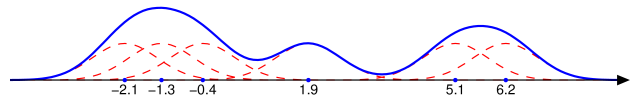
\includegraphics[width=200px]{images/Parzen_window_illustration.png}
\end{center}
\caption{Rouge: courbe en cloche. Bleu: somme des courbes en cloche.
L'estimateur est la moyenne des courbes rouges, ie, la courbe bleue divisée
par $6$}
\end{figure}

Formalisons cette notion. Sachant $n$ point $x_i, i = 1, \dots, n$
dans l'espace $R^d$, une bande passante $H$ de taille $d \times d$, un noyau
$K(x)$, l'estimateur de la densité est:

\begin{equation}
\hat{f}(x) = \frac{1}{n} \sum_{i = 1}^n K_H(x - x_i)
\end{equation}

Pour les noyaux à symétrie circulaire, il suffit de définir le profile du
noyau $k(x)$. On a alors:

\begin{equation}
K(x) = c_{k, d} k (|| x ||^2)
\end{equation}

$x_{k, d}$ est une constante de normalisation strictement positive, permettant
d'assurer la contrainte suivante:

\begin{equation*}
\int_{R^d} K(x) dx = 1
\end{equation*}

\begin{figure}[h]
\begin{center}
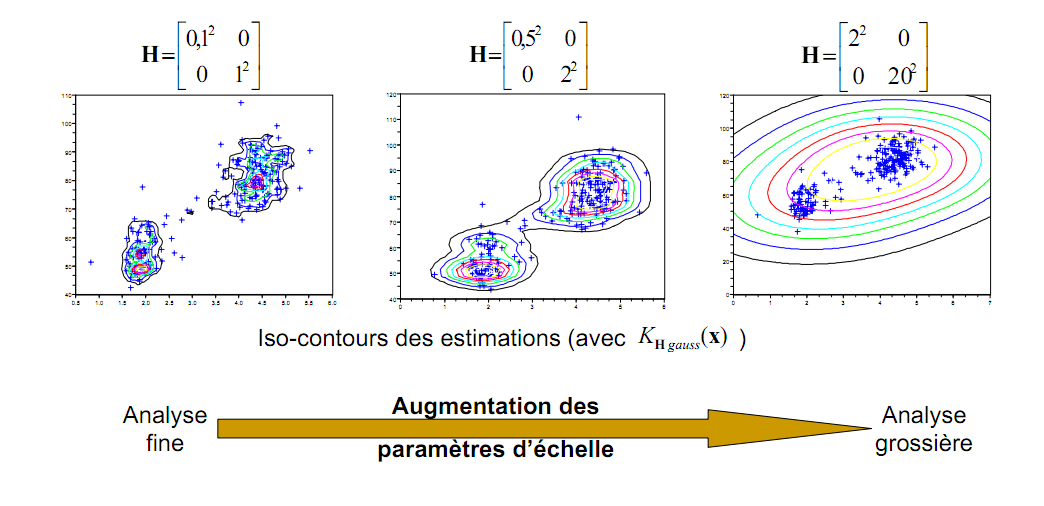
\includegraphics[width=350px]{images/parametre_d_echelle.png}
\end{center}
\caption{Influence des paramètres sur les estimations}
\end{figure}

Si complétement paramétrisée, la bande passante $H$ permet de raffiner
l'estimation. Elle est cependant souvent choisie comme étant diagonale
$H = diag [h_1^2, \dots, h_n^2]$, ou proportionnelle à l'identité $H = h \times
I$. Nous nous restreindrons à ce dernier cas, ce qui permet de ne définir
qu'un seul paramètre. Avec cette contrainte supplémentaire, la densité
s'écrit:

\begin{equation}
\hat{f}(x) = \frac{1}{nh^d} \sum_{i = 1}^n K\(\frac{x - x_i}{h}\)
\end{equation}


\cite{cheng} proposent deux exemples de noyaux:

\begin{itemize}
\item noyau plat:
  \begin{equation*}
  K(x) =  1 if ||x|| \leq 1 else 0
  \end{equation*}
\item noyau gaussian
  \begin{equation*}
  K(x) = \exp \( - || x ||^2 \)
  \end{equation*}
\end{itemize}

\begin{figure}
\begin{center}
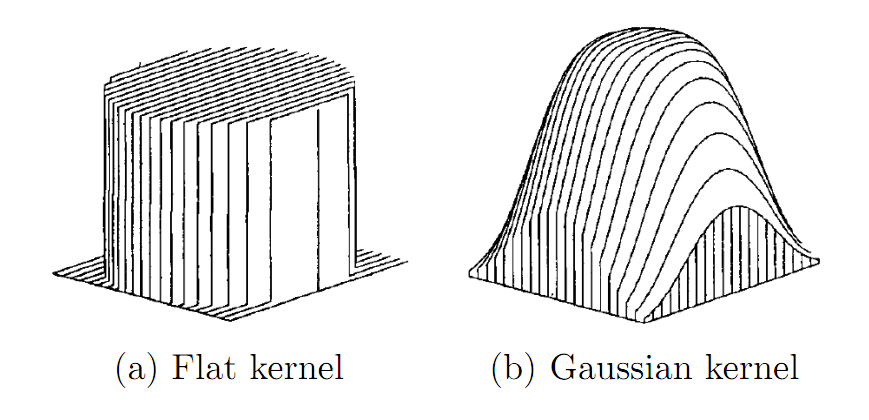
\includegraphics[width=250px]{images/noyaux.png}
\end{center}
\end{figure}

Nous avons maintenant tous les outils pour calculer le gradient de
l'estimateur de densité:

\begin{align*}
\hat{\nabla} f_{h, K}(x) & = & \nabla \hat{f}_{h, K}(x) \\
			 & = & \frac{2 c_{k, d}}{n h^{d + 2}} \sum_{i = 1}^n
			 (x - x_i)  g\( \| \frac{x - x_i}{h}
			 \|^2\) \\
			 & = & \frac{2 c_{k, d}}{n h^{d + 2}} \[ \sum_{i = 1}^n
			 (x - x_i) \] \[ \frac{\sum_{i = 1}^n x_i g\(\|
			 \frac{x - x_i}{y} \|^2\)}{ \sum_{i = 1}^n g \( \|
			 \frac{x - x_i}{h} \|^2\) } - x\]
\end{align*}

avec $g = - k'$. On remarque que le premier terme est proportionnel à
l'estimateur de densité au point $x$ (calculé avec le noyau $G = c_g
g(\|x\|^2)$. Le deuxième terme est le vector mean shift $m$, qui pointe vers
la direction de l'augmentation maximal de densité, et est proportionnal au
gradient de l'estimateur de densité au point $x$, avec le noyau $K$. On peut
donc réécrire l'algorithme mean shift au point $x_i$ tel qu'il suit:

\begin{itemize}
\item Calculer le vecteur meanshft $m(x_i^t)$
\item Déplacer la fenêtre d'estimation de densité $x_i^{t + 1} = x_i^t +
m(x_i^t)$.
\item Itérer jusqu'à converge, ie jusqu'à $\nabla f(x_i) = 0$
\end{itemize}

Nous utiliserons l'implémentation du MeanShift en python de scikit-learn,
(\cite{sklearn}).

\section{Descripteurs pour la segmentation}

Parmi les descripteurs intuitifs d'une image, on peut citer les différents
espaces de couleurs. Des descripteurs de texture peuvent aussi être utilisés,
ainsi qu'une combinaison des descripteurs de couleurs et de texture.

\subsection{Couleurs}

\begin{figure}
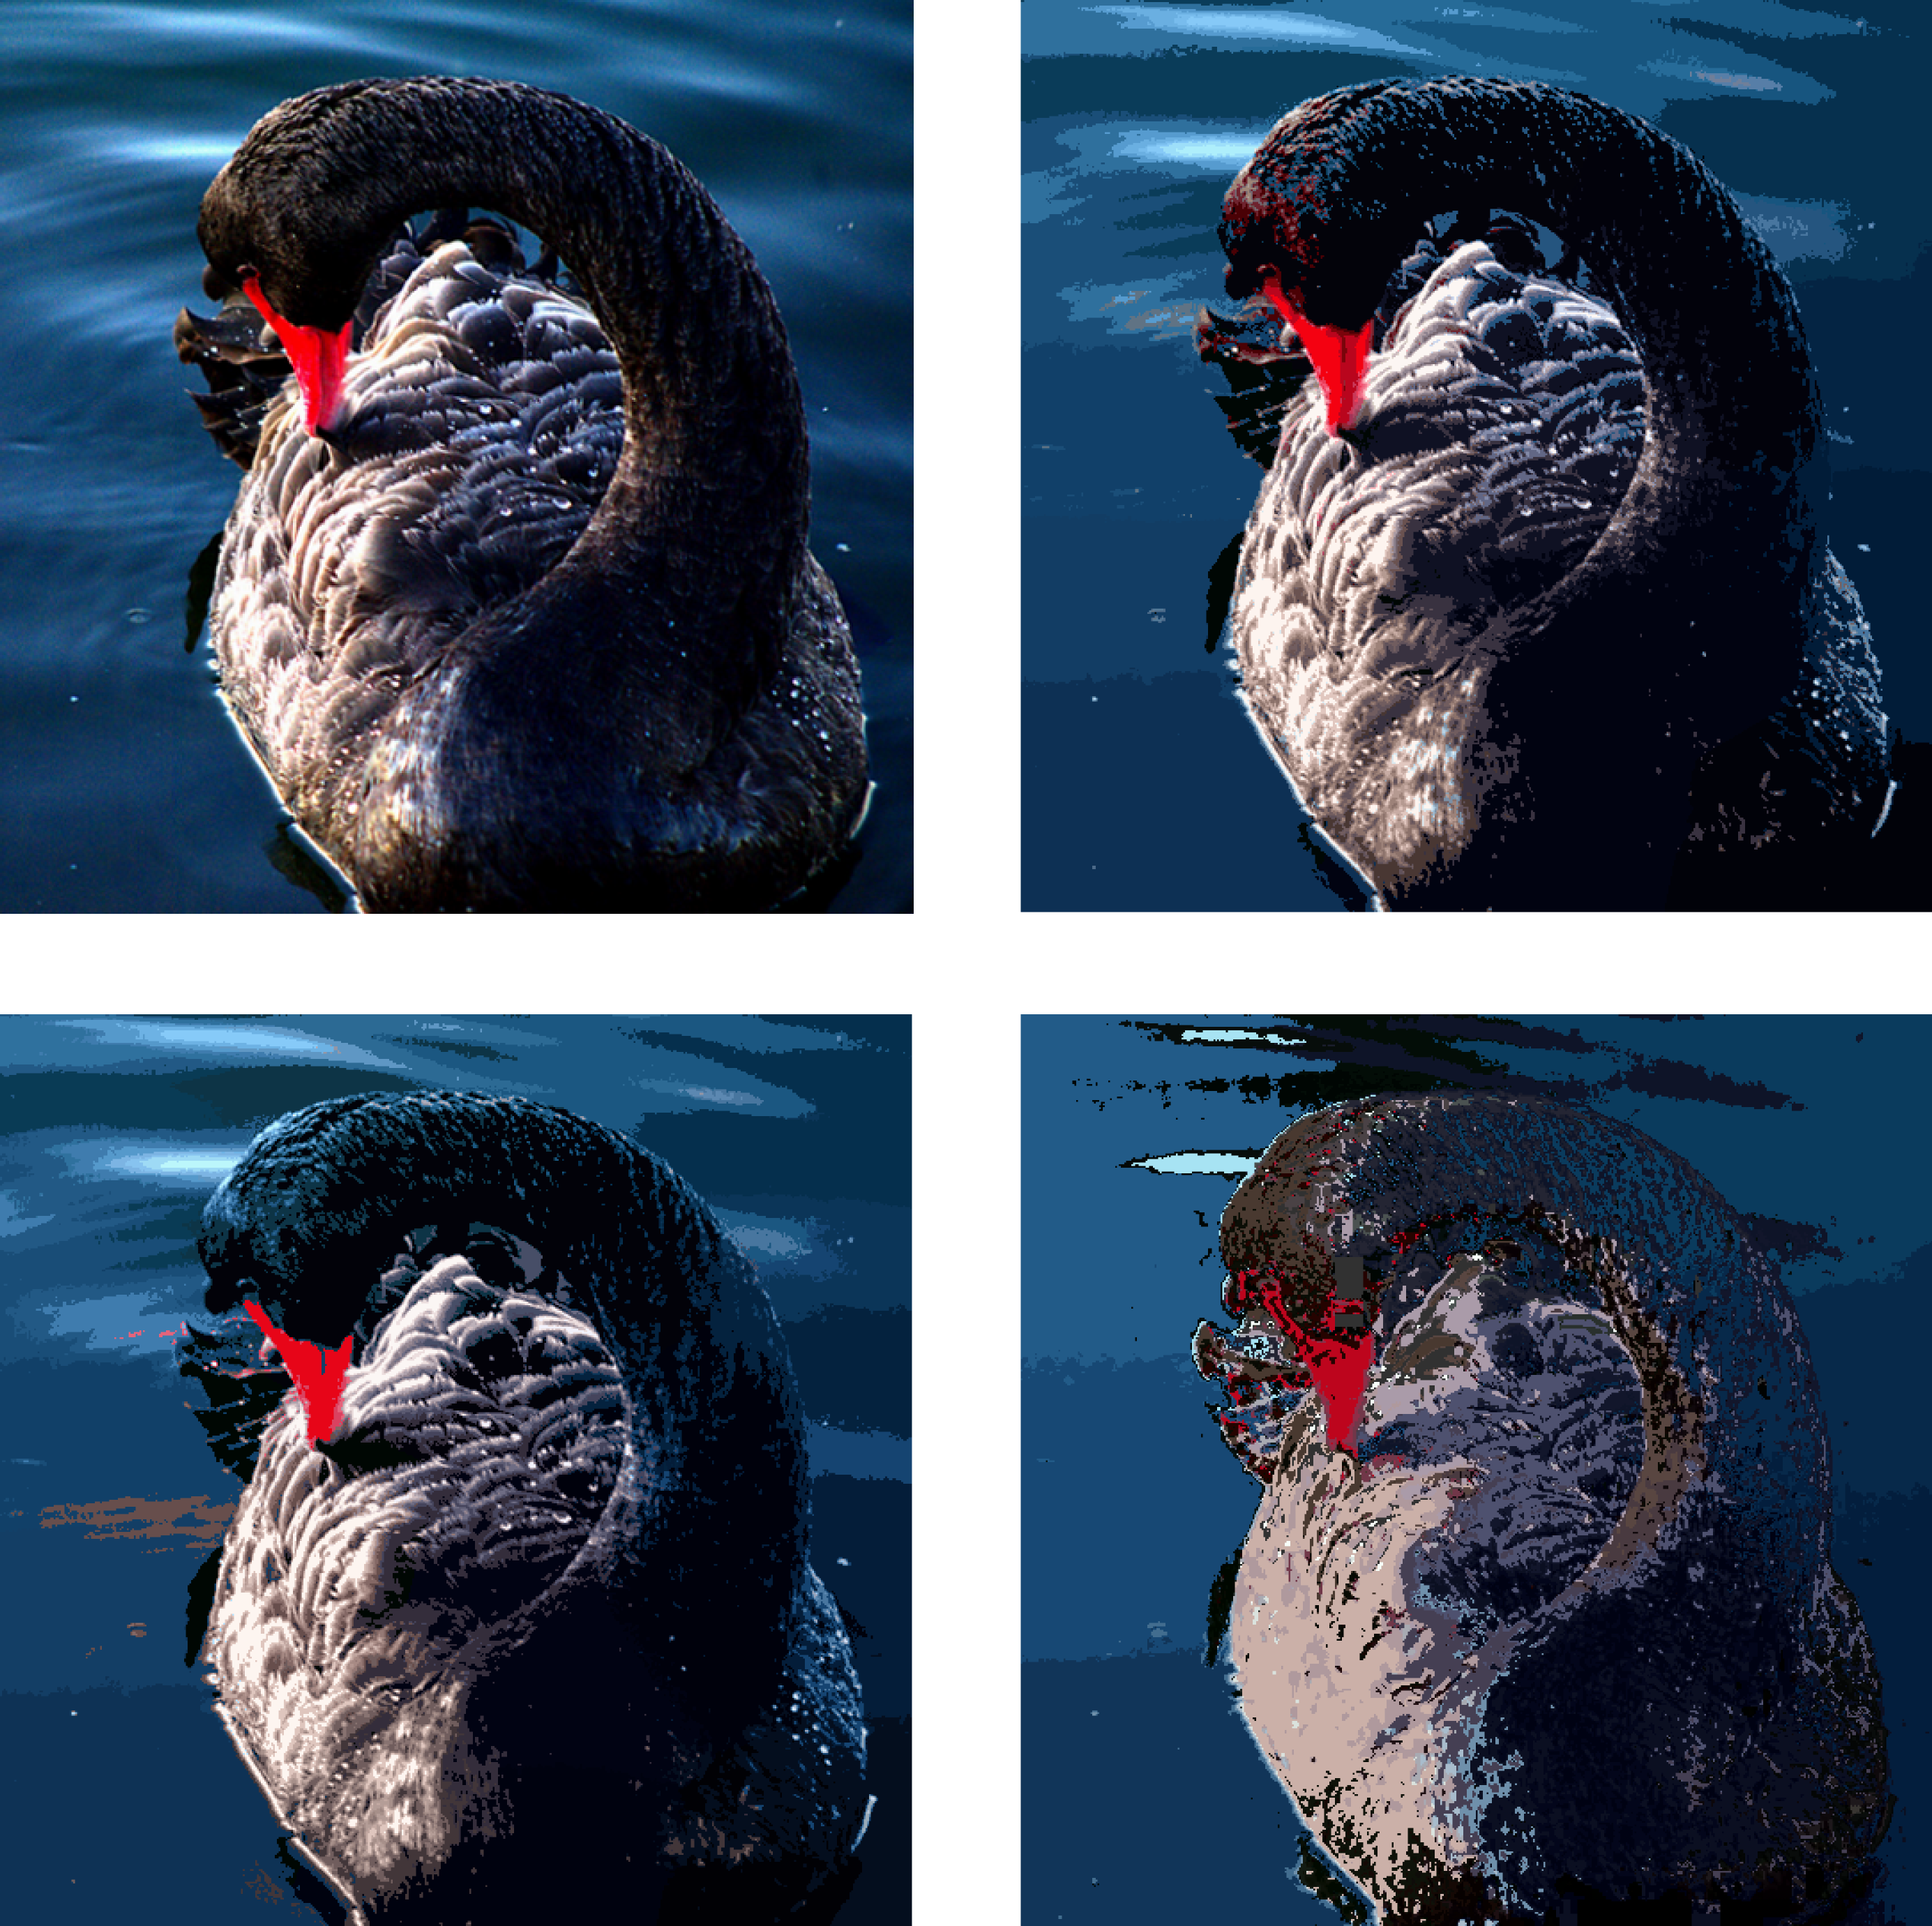
\includegraphics[width=450px]{images/color_black_swan.png}
\caption{Haut gauche - Image originale: Black Swan, 512 * 512, par Agnès
Maillard. Haut gauche - MeanShift RGB - MeanShift HSV - Meanshift XYZ. Les
meanshift sont calculées avec les mêmes paramètres.}
\end{figure}

On dispose de plusieurs espaces de couleurs, que nous pouvons utiliser comme
descripteurs:

\begin{itemize}
\item niveau de gris: le descripteurs le plus simple est certainement le
niveau de gris. Étant d'une dimension, le calcul du meanshift est
particulièrement rapide sur celui-ci. Il est d'un interêt limité.
\item RGB: cet espace corresponds aux couleurs primaires, qui correspondent
aux trois longueurs d'onde auxquelles répondent l'oeil humain.
\item HSV (hue saturation value): cet espace de teinte, saturation et valeur,
est obtenu par une transformatio non linéaire de l'espace de couleur RGB
\item XYZ: cet espace se rapproche vers une description des couleurs conforme
à la vision humain, celui introduisant la notion subjective de la luminance.
\end{itemize}

Nous utilisons la libraire scikits-image pour effectuer les changements
d'espace de couleur.

\subsection{Textures}

\begin{figure}
\label{bins}
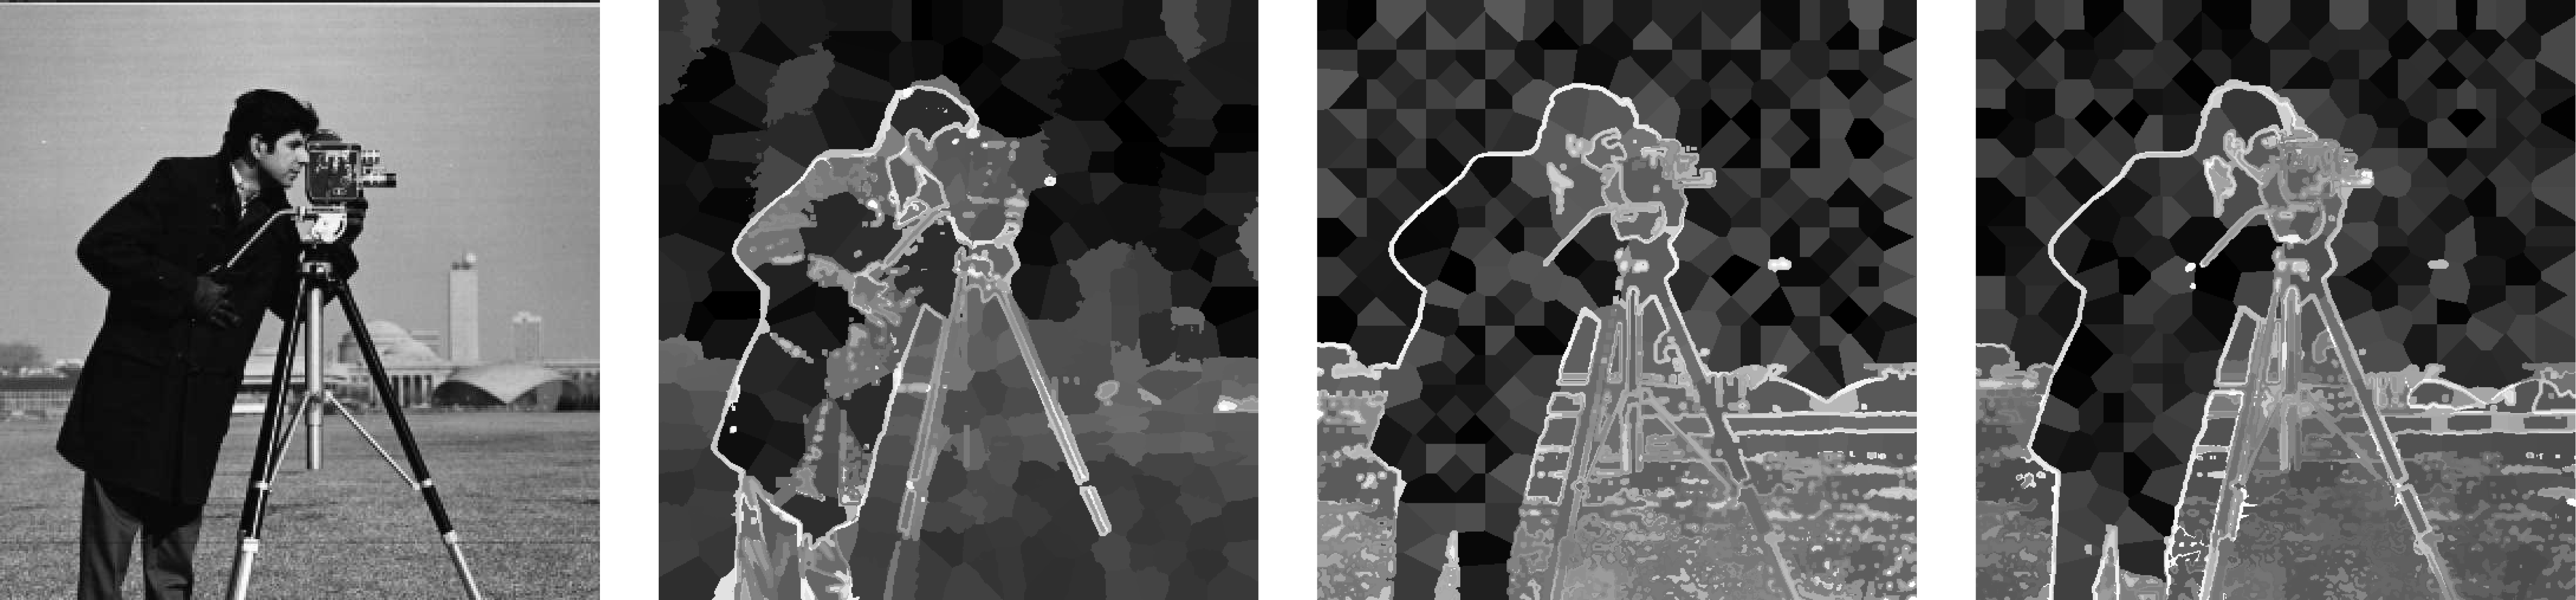
\includegraphics[width=500px]{images/cameraman.png}
\caption{Cameraman, segmentée avec plusieurs descripteurs de texture
(histogramme de niveaux de gris. Image original, MeanShift sur histogramme 
quantifié sur 16bins, 4bins et 2bins et descripteurs spatiaux)}
\end{figure}

Il existe plusieurs manières de représenter les textures. Nous nous limiterons
ici aux textures microscopiques: nous ignorerons donc le cas des textures
macroscopiques, dont nous pouvons distinguer les éléments géométriques
(pommes, galets etc...). Il est cependant bon de rappeler qu'une texture
macroscopique peut devenir microscopique avec un changement d'échelle.

Une texture microscopique est très bien représentée par les statistiques de
premier ordre:
\begin{itemize}
\item Moyenne: $\mu(I) = \frac{1}{N^2} \sum_z I(z)$
\item Variance: $\sigma^2(I) = \frac{1}{N^2} \sum_z (I(z) - \mu)$
\item Energie: $E(I) = \frac{1}{N^2} \sum_z (I(z)^2$
\item Entropie: $H(I) = - \sum_{g = 1}^G f(g) \log(f(g))$
\end{itemize}

Ces quantités ne dépendent que de l'histogramme de l'image, et peuvent donc
prendre des valeurs arbitraires sous l'effet d'un changement de constraste.
Ces descripteurs  sont estimés sur des voisinages bornées, avec des patchs
glissants: ils sont donc approximativement liés à une localisation.

Nous utiliserons des histogrammes de niveaux de gris, calculés sur des petits
patchs d'image de taille $5 \times 5$. Ces histogrammes peuvent être
quantifiés sur un nombre variable de bins afin d'avoir des descripteurs
variés. \ref{bins} montre le résultat d'une segmentation en utilisant des
descripteurs différents, de tailles variants entre $5$ et $19$ éléments.

\begin{figure}[h]
\begin{center}
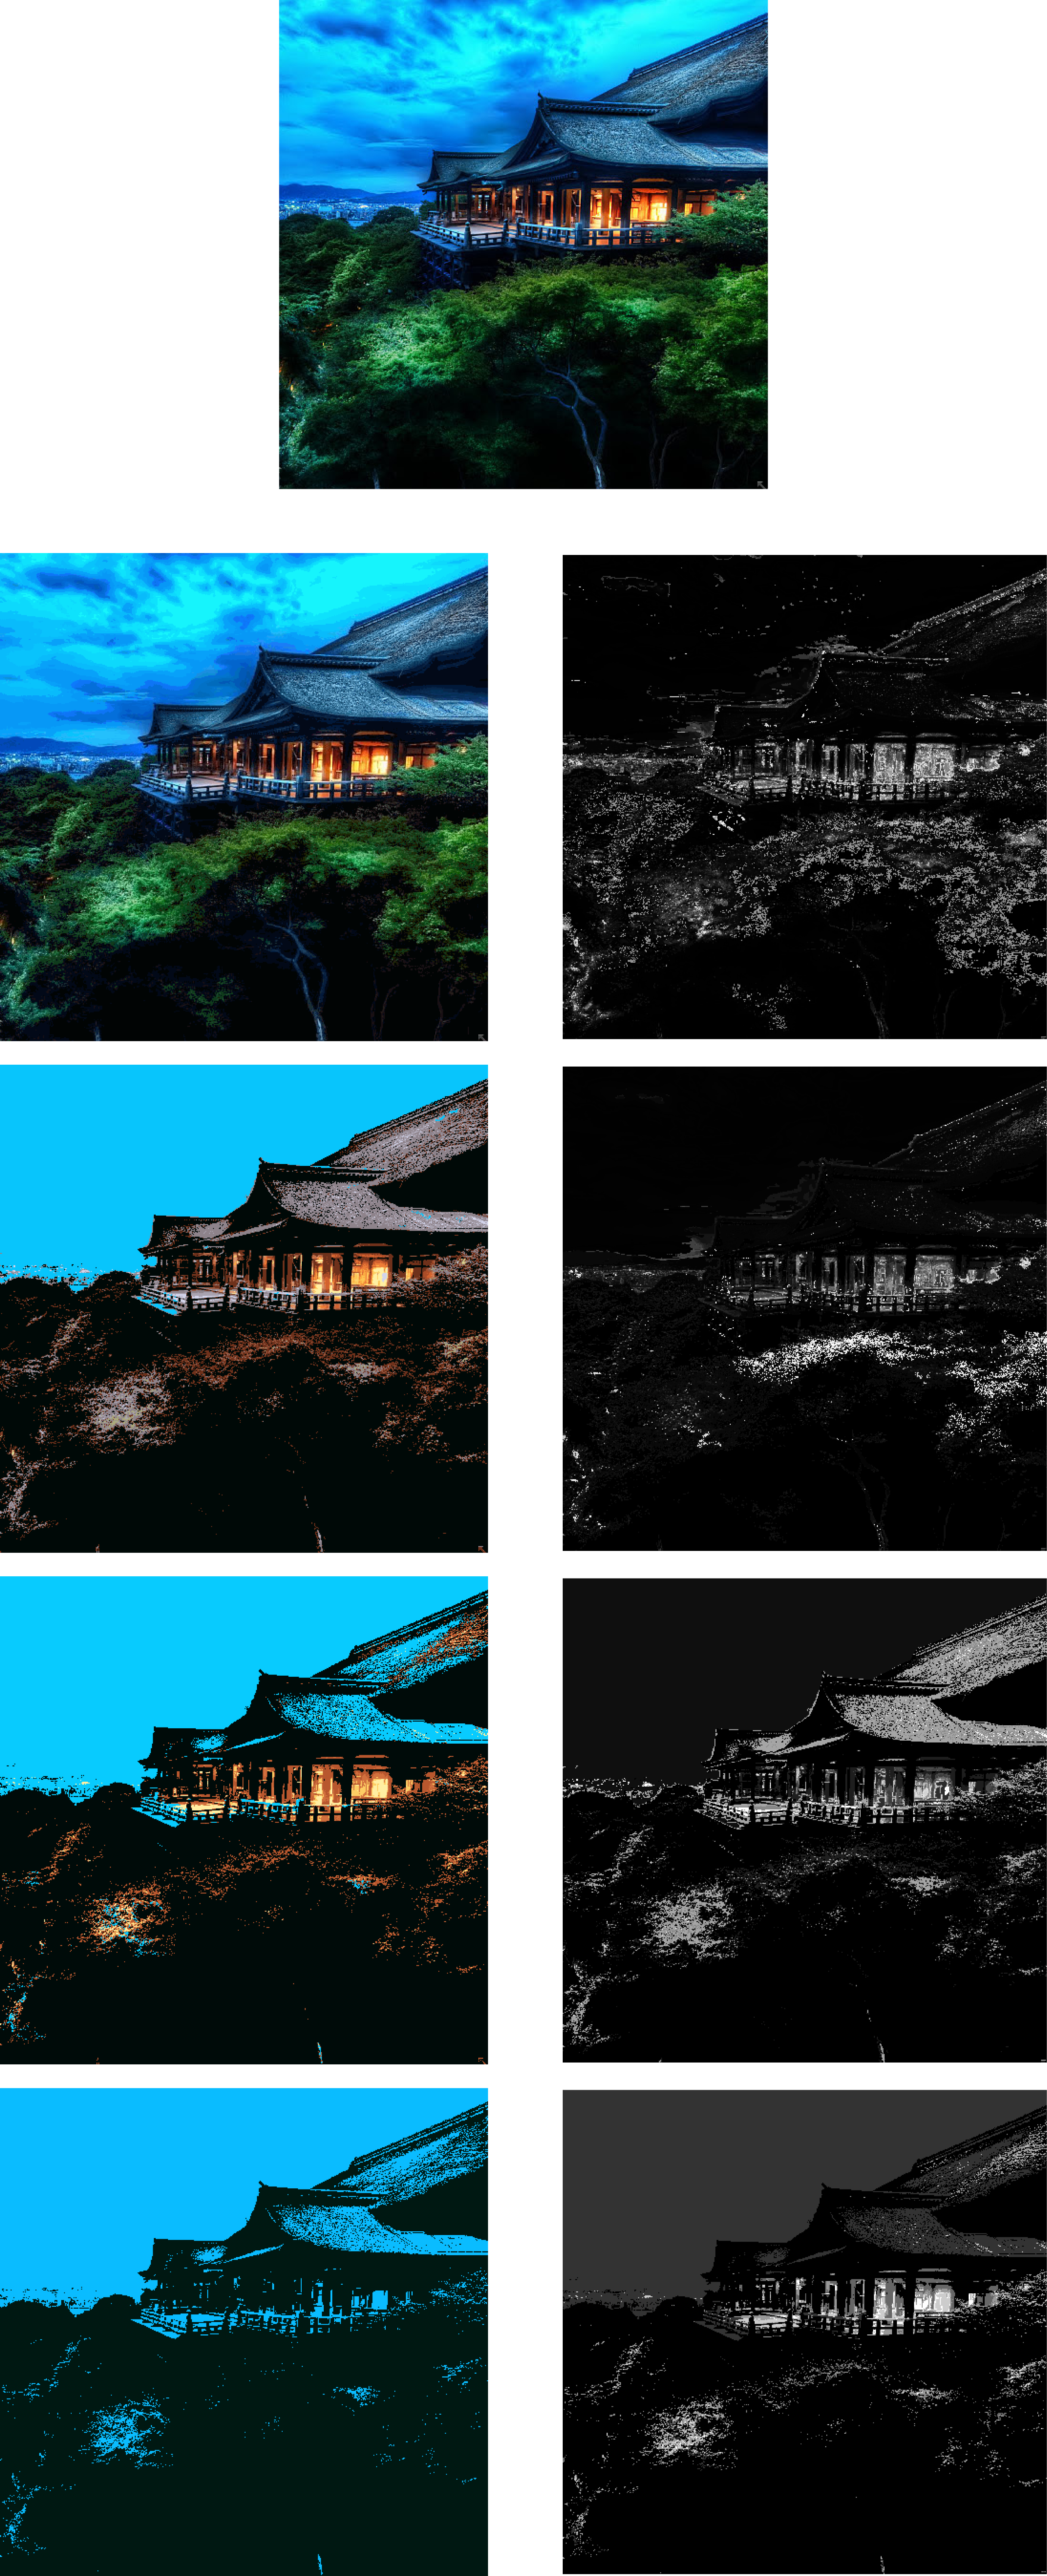
\includegraphics[width=200px]{images/all_chinese_temple.png}
\end{center}
\caption{Chinese Temple (HDR) by Trey Ratcliff, segmented using RGB (left) and
texture (right), with varying quantiles}
\end{figure}

\begin{figure}[h]
\label{lena}
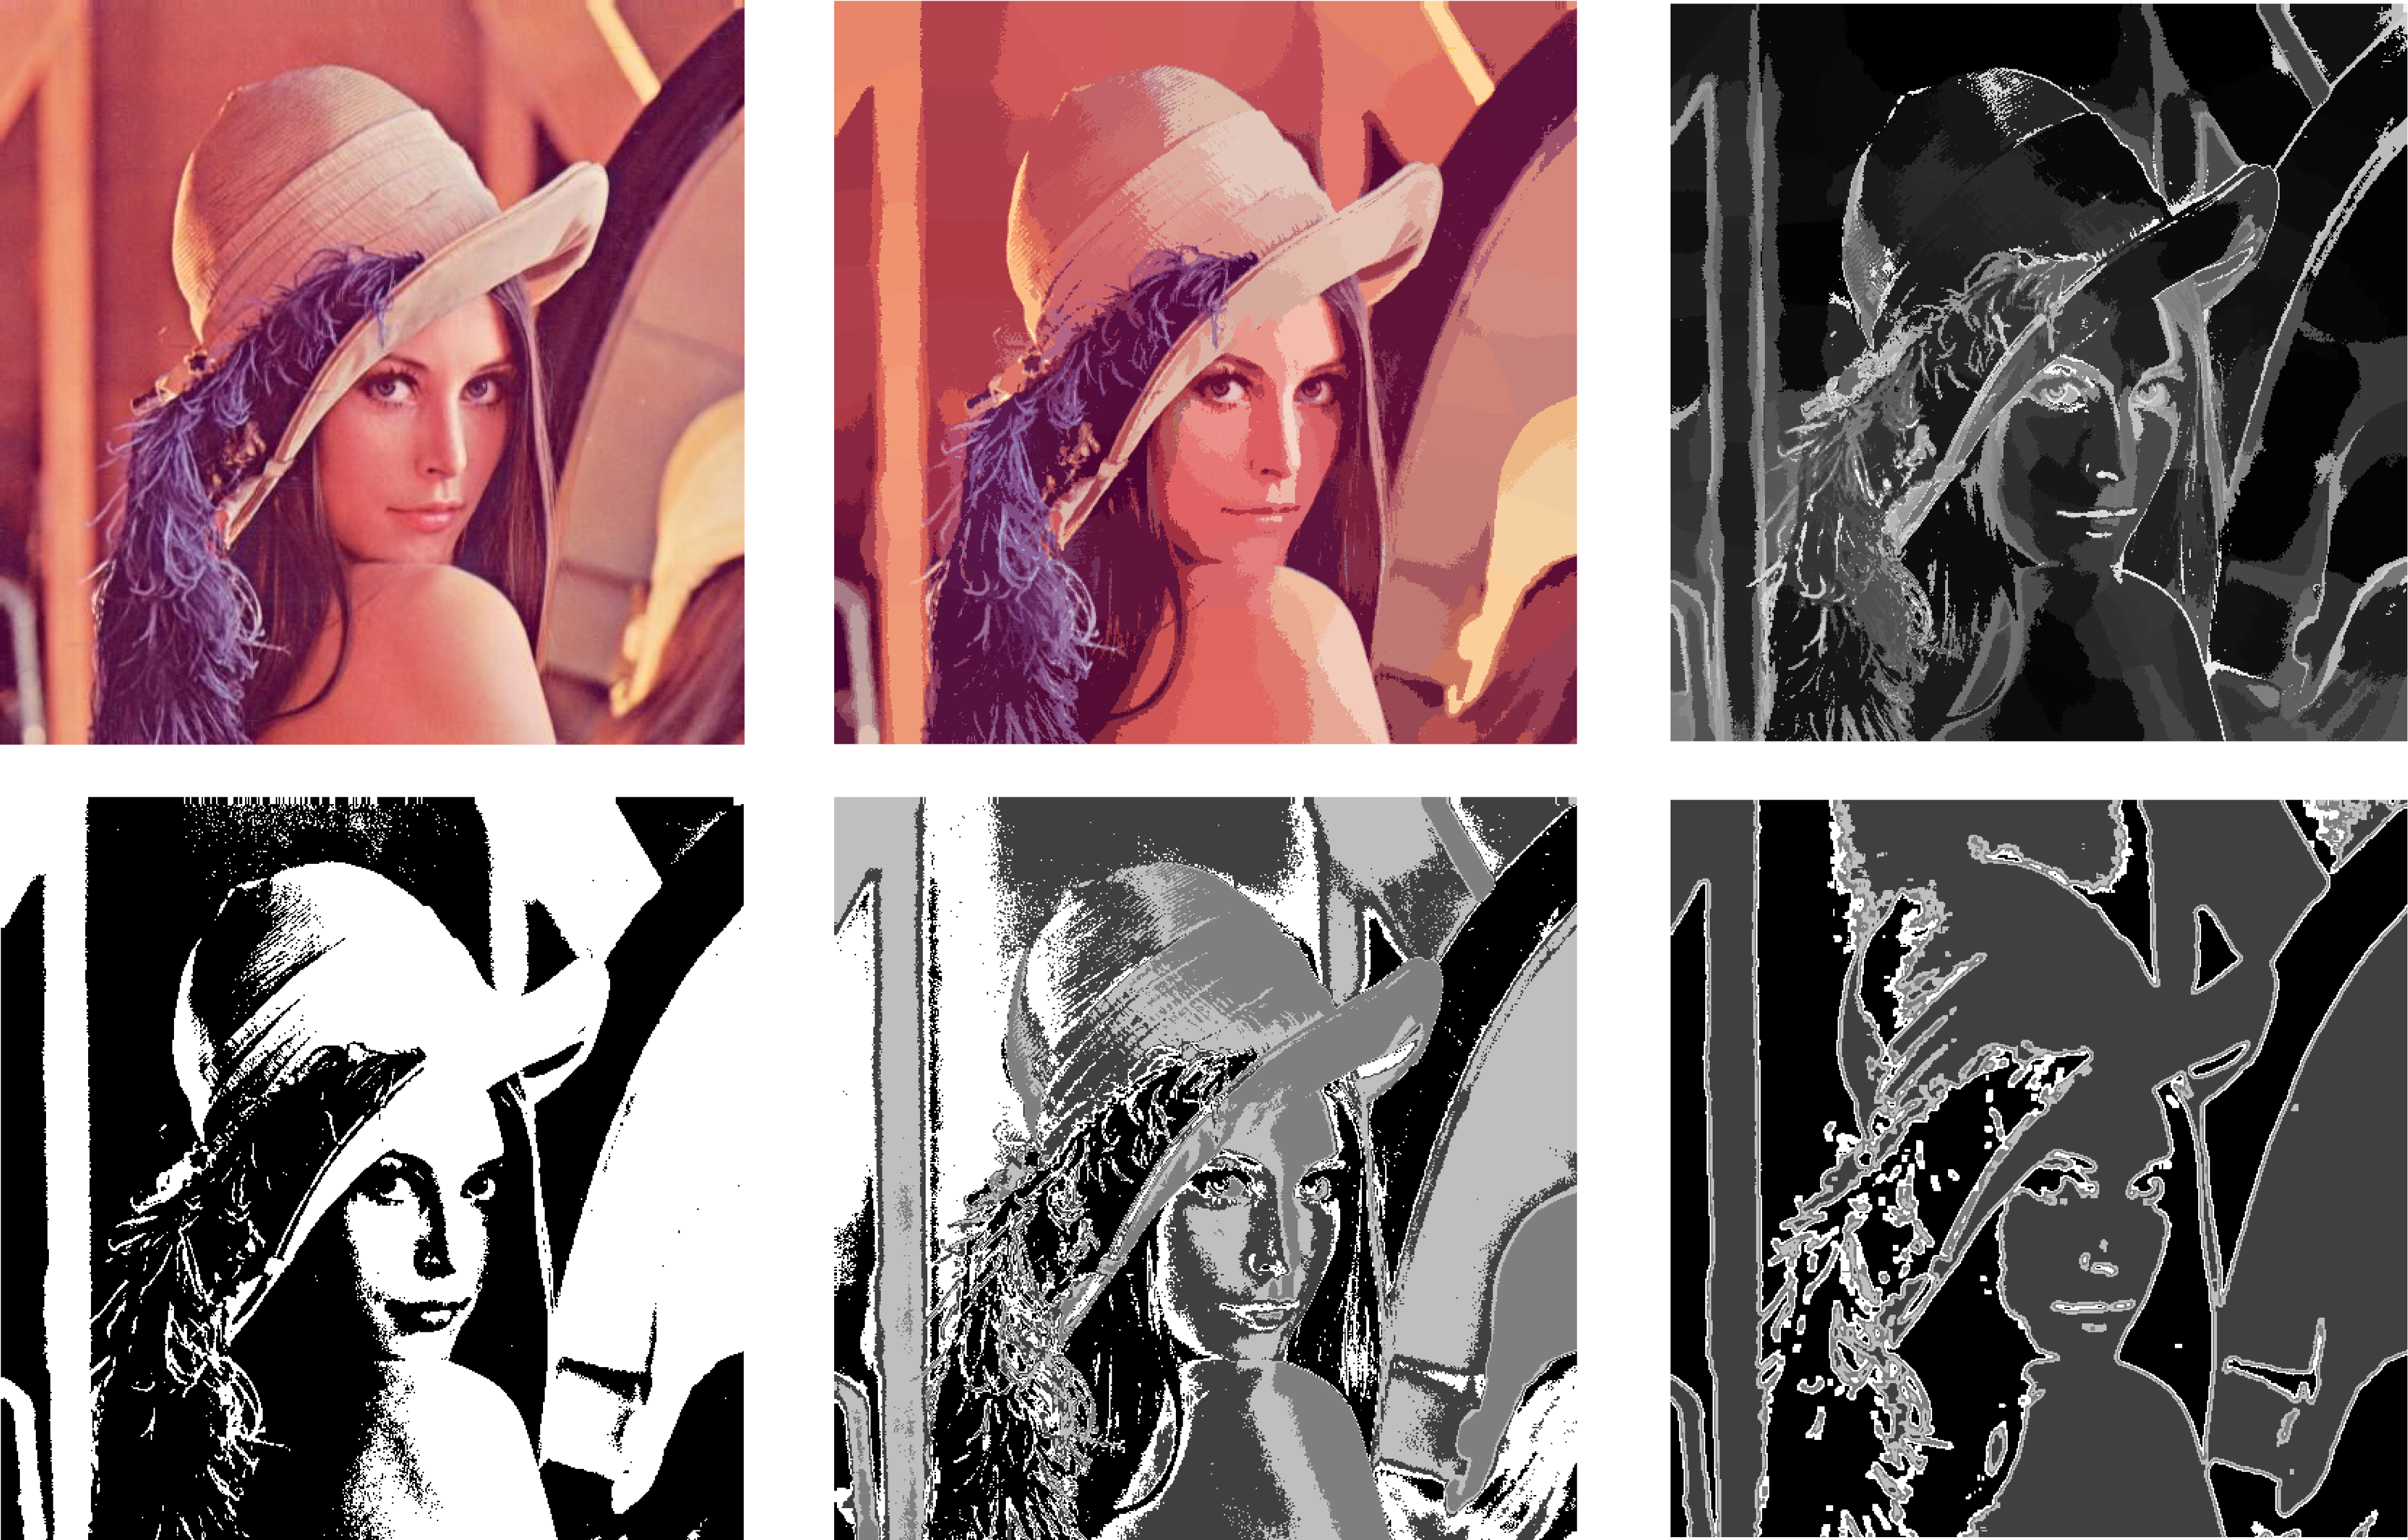
\includegraphics[width=400px]{images/all_lena.png}
\caption{Lena - Haut gauche: image originale - haut milieu: image segmentée à
l'aide du meanshift, dans l'espace des descripteurs RGB + spatial - haut
droit: image segmentée avec le meanshit dans l'espace des descripteurs de
textures (6bins), des couleurs (RGB) et spatiale - bas droite: image segmentée
avec le k-means, $k = 2$, dans l'espace des couleurs et spatiale - bas milieu:
image segmentée avec le k-means, $k = 5$, dans l'espace des couleurs RGB et
spatial - bas droite: image segmentée avec le k-means, $k = 5$, dans l'espaces
des descripteurs de textures (6bins), des couleurs (RGB) et spatiale.}
\end{figure}

\newpage
\section{Conclusion}

\begin{wrapfigure}{l}{0.4\textwidth}
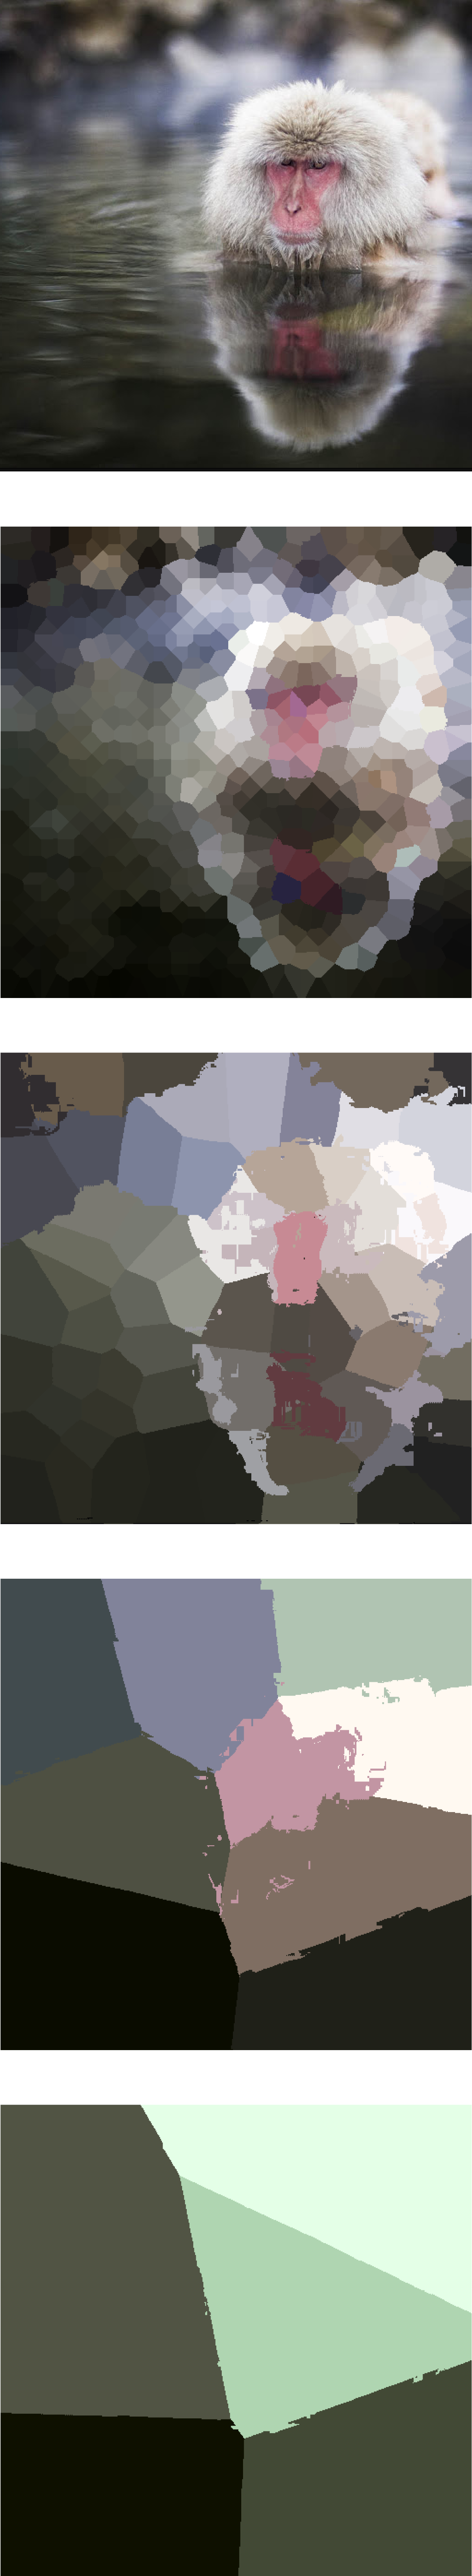
\includegraphics[width=110px]{images/white_baboon.png}
\end{wrapfigure}

Malgré la volonté de \cite{my_article} de limiter le nombre de paramètre à
trouver, le meanshift nécessite de trouver la bande passante ou le quantile le
plus performant. Ne pas le choisir correctement peut mener à des résultats
catastrophiques. Dans certains cas, il est donc plus simple d'utiliser le
k-means, dont le paramètre $k$ correspond au nombre de cluster, et est donc
plus intuitif à trouver (Figure \ref{lena}). \\
Cependant, il existe des moyens d'estimer la bande passante, comme décrit dans
\cite{fastnonparametric}, afin d'avoir un algorithme non paramétrique.

\bibliography{biblio}
\end{document}
